\chapter{Pruebas y Validación} % Main chapter title
\label{Chapter6}
\lhead{Capítulo 6. \emph{Pruebas y Validación}}
\setstretch{1.1} % Line spacing of 1.1
En el presente capítulo se describen los procedimientos de prueba para los requerimientos descritos en el cuadro \ref{table:req_user}. Cada uno de los cuadros visibles a continuación describe el objetivo de la prueba, el procedimiento, el resultado esperado y el estado final, que indican si la prueba se realizó de forma exitosa o no. Por último, en el capítulo se encuentra una matriz de trazabilidad que permite relacionar los requerimientos de usuario con los requerimientos funcionales y asociar cada uno con su caso de prueba correspondiente.
\section{Validación de los requerimientos de usuario}
\renewcommand{\tabularxcolumn}[1]{>{\arraybackslash}m{#1}}
% prueba req1
\begin{table}[H]
    \rowcolors{2}{gray!20}{white}
    \begin{tabularx}{\textwidth}{|m{3cm}|X|}
    \hline
    Id & TC-01\\
    \hline
    Título & Creación de un acta nueva en el Blockchain \\
    \hline
    Objetivo & Demostrar el funcionamiento correcto de la carga de actas al Blockchain.\\
    \hline
    Procedimiento & \begin{enumerate}
        \item El usuario debe dirigirse hacia la página y hacer clic en el cuadro con el título ``Subir acta nueva''.
        \item Luego debe ingresar el acta en el campo de texto previsto y hacer clic en el botón ``Subir acta''.
        \item Después de un tiempo de espera una alerta indicará si el acta pudo ser subida exitosamente o no.
    \end{enumerate}\\
    \hline
    Resultados esperados & Luego de un tiempo de espera, un cartel indicará el éxito de la operación. En el caso que el acta fue subida anteriormente y ya existe, indicará con un mensaje de error que el acta no pudo ser agregada.\\
    \hline
    Estado & Aprobado\\
    \hline
    \end{tabularx}
    \caption{Caso de prueba TC-01}
\end{table}
%prueba req 2
\begin{table}[H]
\rowcolors{2}{gray!20}{white}
\begin{tabularx}{\textwidth}{|m{3cm}|X|}
\hline
Id & TC-02\\
\hline
Título & Consulta de un acta en el Blockchain \\
\hline
Objetivo & Recuperar el acta del Blockchain con sus renglones en formato de \textit{hash}, tal como se subió.\\
\hline
Procedimiento & \begin{enumerate}
    \item El usuario debe dirigirse hacia la página y hacer clic en el cuadro con el título ``Consultar acta''.
    \item Luego debe ingresar el id del acta en el campo de texto previsto y hacer clic en el botón ``Obtener''.
\end{enumerate}\\
\hline
Resultados esperados & En el caso de que el acta exista, el contenido de la misma aparece debajo del botón, indicando los campos de la cabecera y los renglones. En el caso de no existir el acta, una alerta proporciona dicha información al usuario. Capturas de ambos casos se encuentran en las figuras \ref{fig:query_success} y \ref{fig:query_failure}.\\
\hline
Estado & Aprobado\\
\hline
\end{tabularx}
\caption{Caso de prueba TC-02}
\end{table}

\begin{figure}[H]
    \center{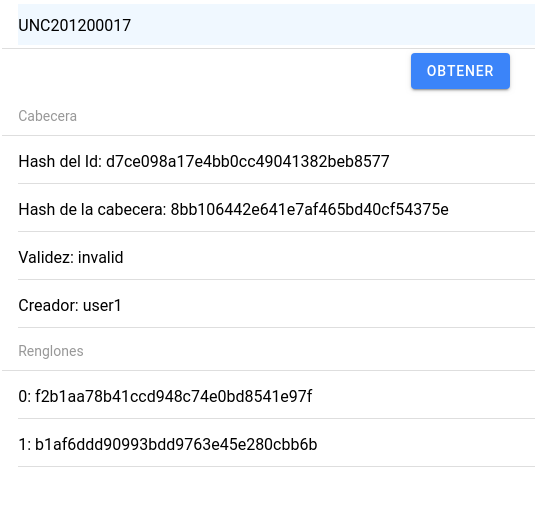
\includegraphics[width=0.8\linewidth]{Figures/Selection_234.png}}
    \caption{Alertas de notificación sobre el éxito o fracaso de una operación.}
    \label{fig:query_success}
\end{figure}

\begin{figure}[H]
    \center{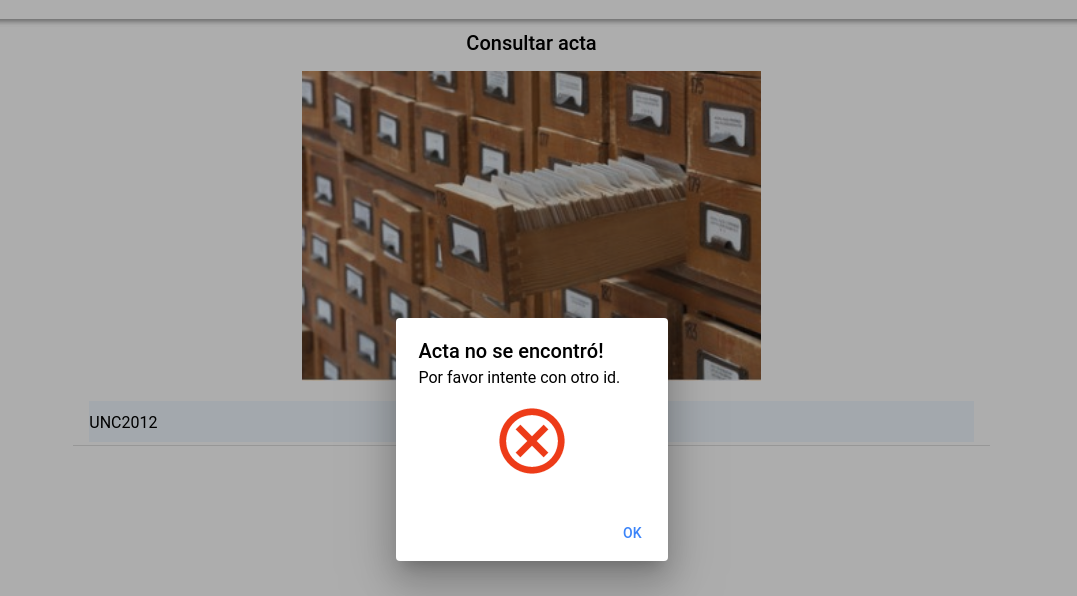
\includegraphics[width=0.8\linewidth]{Figures/Selection_233.png}}
    \caption{Alertas de notificación sobre el éxito o fracaso de una operación.}
    \label{fig:query_failure}
\end{figure}

%prueba req 3
\begin{table}[H]
\rowcolors{2}{gray!20}{white}
\begin{tabularx}{\textwidth}{|m{3cm}|X|}
\hline
Id & TC-03\\
\hline
Título & Validación de una nota con el Blockchain \\
\hline
Objetivo & Obtener información sobre la validez o invalidez de una nota.\\
\hline
Procedimiento & \begin{enumerate}
    \item El usuario debe dirigirse hacia la página y hacer clic en el cuadro con el título ``Validar nota''.
    \item Luego debe ingresar toda la información correspondiente en el campo de texto previsto y hacer clic en ``Validar''.
    \item Después de un tiempo de espera una alerta indicará si la nota es válida o no.
\end{enumerate}\\
\hline
Resultados esperados & Un cartel indica si la nota es válida, si no es válida o que el acta en el cual se tenía que encontrar la nota no existe.\\
\hline
Estado & Aprobado\\
\hline
\end{tabularx}
\caption{Caso de prueba TC-03}
\end{table}

%prubea requerimiento 4
\begin{table}[H]
\rowcolors{2}{gray!20}{white}
\begin{tabularx}{\textwidth}{|m{3cm}|X|}
\hline
Id & TC-04\\
\hline
Título & Validación de una historia académica \\
\hline
Objetivo & Obtener información sobre la validez o invalidez de una historia académica.\\
\hline
Procedimiento & \begin{enumerate}
    \item El usuario debe dirigirse hacia la página y hacer clic en el cuadro con el título ``Validar historia académica''.
    \item Luego debe ingresar toda la información correspondiente en el campo de texto previsto y hacer clic en ``Validar''.
    \item Después de un tiempo de espera, la página indicará si la historia académica es válida o no.
\end{enumerate}\\
\hline
Resultados Esperados & Como en el caso de la validación de una sola nota, un cartel indica la validez o invalidez de la historia académica. Por debajo del botón ``Validar'' aparece una lista con los ids de las actas que se consultó y el resultado por cada acta. En la figura \ref{fig:academic_history_fail} se puede ver un ejemplo donde no se logró validar una historia académica, junto con el detalle de los errores de las notas que no se lograron validar. \\
\hline
Estado & Aprobado\\
\hline
\end{tabularx}
\caption{Caso de prueba TC-04}
\end{table}

\begin{figure}[H]
    \center{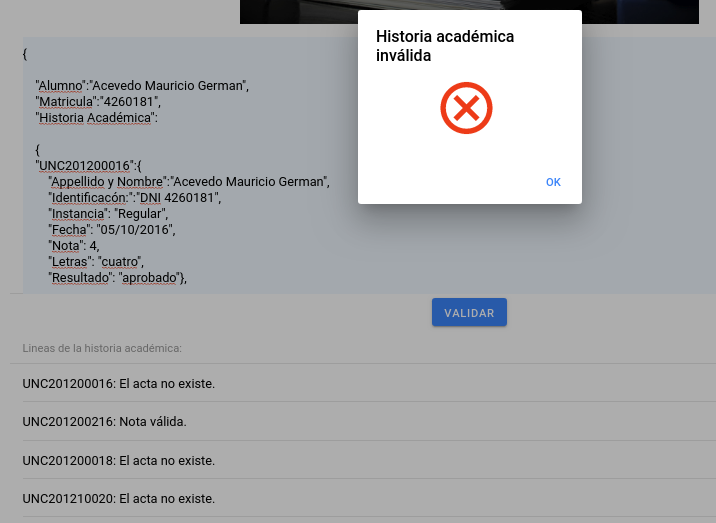
\includegraphics[width=0.8\linewidth]{Figures/Selection_235.png}}
    \caption{Caso de una historia académica inválida.}
    \label{fig:academic_history_fail}
\end{figure}

%prubea requerimiento 5
\begin{table}[H]
\rowcolors{2}{gray!20}{white}
\begin{tabularx}{\textwidth}{|m{3cm}|X|}
\hline
Id & TC-05\\
\hline
Título & Revocar un acta \\
\hline
Objetivo & Corroborar el funcionamiento correcto del sistema al revocar una acta.\\
\hline
Procedimiento & \begin{enumerate}
    \item El usuario debe dirigirse hacia la página y hacer clic en el cuadro con el título ``Revocar acta''.
    \item Luego debe ingresar toda la información correspondiente en el campo de texto previsto y hacer clic en el botón ``Revocar acta''.
    \item Después de un tiempo de espera, la página indicará si el acta pudo ser revocada o no.
\end{enumerate}\\
\hline
Resultados Esperados & En el caso de una revocación inválida, es decir, en el caso que el acta a revocar no existe o ya es inválida, el sistema devuelve un error. Si se puede revocar al acta, el sistema avisa después de un tiempo de espera que el acta pudo ser revocada correctamente.\\
\hline
Estado & Aprobado\\
\hline
\end{tabularx}
\caption{Caso de prueba TC-05}
\end{table}


%prueba req 6
\begin{table}[H]
\rowcolors{2}{gray!20}{white}
\begin{tabularx}{\textwidth}{|m{3cm}|X|}
\hline
Id & TC-06\\
\hline
Título & Consulta de las actas rectificadas\\
\hline
Objetivo & Recuperar información sobre todas las actas rectificadas existentes en el Blockchain.\\
\hline
Procedimiento & \begin{enumerate}
\item El usuario debe dirigirse hacia la página y hacer clic en el cuadro con el título ``Obtener actas rectificadas''.
\item En la página, debe hacer clic en el botón ``Obtener actas rectificadas''.
\end{enumerate}\\
\hline
Resultados esperados & En el caso de no existir ningún acta rectificada, la página muestra un texto indicando lo mismo. Si existen actas rectificadas, en una lista se detallan id, \textit{hash} del id, \textit{hash} de la cabecera, la validez del acta como el usuario que lo creó. \\
\hline
Estado & Aprobado\\
\hline
\end{tabularx}
\caption{Caso de prueba TC-06}
\end{table}

\lstset{
  frame=none
}
%prueba 7
\begin{table}[H]
    \rowcolors{2}{gray!20}{white}
    \begin{tabularx}{\textwidth}{|m{3cm}|X|}
    \hline
    Id & TC-07\\
    \hline
    Título & Presencia de Organizaciones y CA's\\
    \hline
    Objetivo & Verificar que existen los \textit{peers} y autoridades de certificación especificados en los requerimientos.\\
    \hline
    Procedimiento & \begin{enumerate}
    \item En la máquina de desarrollo local, ejecutar el comando 
    \begin{lstlisting}^^J
        $ docker ps^^J
    \end{lstlisting}
    \item En el cluster de Kubernetes, ejecutar el comando
    \begin{lstlisting}^^J
        $ kubectl get pods^^J
    \end{lstlisting}
    \end{enumerate}\\
    \hline
    Resultados esperados & Los contenedores o \textit{pods} que están presentes se pueden ver también en la figura \ref{fig:all_containers}: Se pueden encontrar \textit{peer0} como \textit{peer1} de cada organización y los tres contenedores que funcionan como una autoridad de certificación.\\
    \hline
    Estado & Aprobado\\
    \hline
    \end{tabularx}
    \caption{Caso de prueba TC-07}
    \end{table}

\begin{figure}[H]
    \center{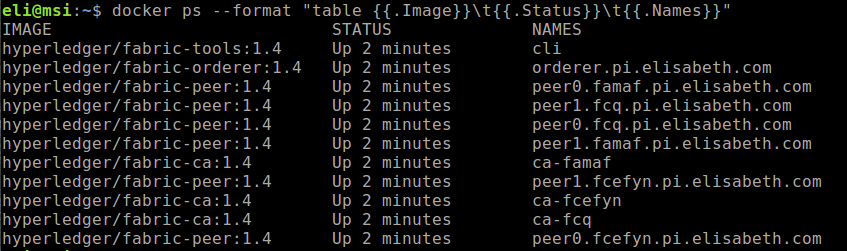
\includegraphics[width=1.0\linewidth]{Figures/Selection_237.png}}
    \caption{Los contenedores que deben estar presentes para cumplir con los requerimientos RF-BC-01 y RF-BC-03. }
    \label{fig:all_containers}
\end{figure}

%prueba 8
\begin{table}[H]
    \rowcolors{2}{gray!20}{white}
    \begin{tabularx}{\textwidth}{|m{3cm}|X|}
    \hline
    Id & TC-08\\
    \hline
    Título & Traducción de la página al inglés\\
    \hline
    Objetivo & Verificar que el \textit{frontend} está disponible en los idiomas inglés y español.\\
    \hline
    Procedimiento & \begin{enumerate}
    \item En la máquina de desarrollo local, ingresar la URL donde está funcionando la aplicación de Angular, en este caso, \textit{http://localhost:8100/home}.
    %\item Para el caso del despliege de Kubernetes, dirigirse hacía el dominio al cual está apuntando el ingrés del cluster.
    \item En la esquina superior derecha de la página, se encuentran una bandera española y una bandera estadounidense. El idioma por defecto es español: Para cambiar al inglés, es necesario hacer clic en la bandera estadounidense.
    \end{enumerate}\\
    \hline
    Resultados esperados & El idioma de toda la página cambia del español al inglés y vice versa al elegir la bandera correspondiente. En la figura \ref{fig:language_change} puede ver el cambio para el caso del título en la página principal.\\
    \hline
    Estado & Aprobado\\
    \hline
    \end{tabularx}
    \caption{Caso de prueba TC-08}
    \end{table}

    \begin{figure}[H]
        \center{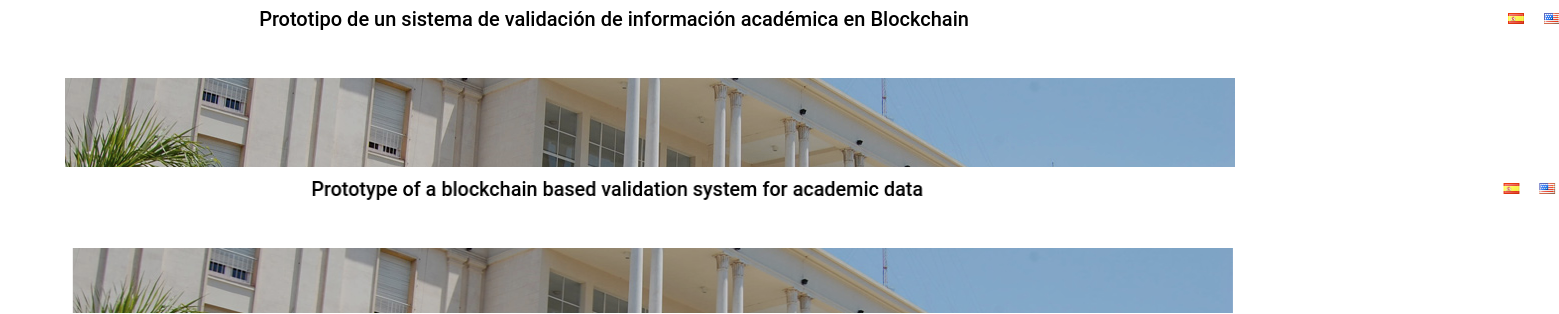
\includegraphics[width=1.0\linewidth]{Figures/Selection_238.png}}
        \caption{Prueba de cambio de idioma en la página principal.}
        \label{fig:language_change}
    \end{figure}

% prubea 9
\begin{table}[H]
    \rowcolors{2}{gray!20}{white}
    \begin{tabularx}{\textwidth}{|m{3cm}|X|}
    \hline
    Id & TC-09\\
    \hline
    Título & Prueba de la página de ayuda\\
    \hline
    Objetivo & Comprobar que un usuario sin conocimiento previo del uso de la página sea capaz de utilizarla.\\
    \hline
    Procedimiento & \begin{enumerate}
    \item Guiar al usuario a la página de ayuda y pedir que lea cuidadosamente las instrucciones.
    \item Pedir al usuario que agregue un acta nueva según las instrucciones y que luego valide una nota de dicha acta. 
    \end{enumerate}\\
    \hline
    Resultados Esperados & Suponiendo el correcto funcionamiento de frontend, API y Blockchain, el usuario no debe tener ningún inconveniente en realizar lo pedido. Para el caso de personas que no tienen ningún conocimiento previo de programación, se anticipan confusiones con la redacción del acta en formato JSON.\\
    \hline
    Estado & Aprobado\\
    \hline
    \end{tabularx}
    \caption{Caso de prueba TC-09}
    \end{table}
\section{Matriz de trazabilidad}
En la matriz visible a continuación se relacionan todos los requerimientos planteados con los casos de test descritos en la sección anterior, con la finalidad de obtener una visión general que todos los requerimientos fueron testeados exitosamente. Los requerimientos no funcionales RNF-01 (El sistema debe contar con pruebas y tests integrales de los seis requerimientos de usuario.) y RNF-02 (El código del \textit{chaincode} debe estar escrito en Golang, la API debe desarrollarse en Node.js y para la interfaz gráfica se debe usar Typescript.) no figuran en la tabla, ya que establecen metodologías y herramientas de trabajo.

\newcommand*\rot{\rotatebox{90}}
\newcommand*\OK{\ding{51}}


\begin{table}[h]
    \begin{adjustwidth}{-1.5cm}{}
    \begin{tabular}{c|cccccc|cccccc|ccccc|cc|}
        &
        \rot{RF-BC-01 } &
        \rot{RF-BC-02 } &
        \rot{RF-BC-03 } &
        \rot{RF-BC-04 } &
        \rot{RF-BC-05 } &
        \rot{RF-BC-06 } &
        \rot{RF-API-01 } &
        \rot{RF-API-02 } &
        \rot{RF-API-03 } &
        \rot{RF-API-04 } &
        \rot{RF-API-05 } &
        \rot{RF-API-06 } &
        \rot{RF-GUI-01 } &
        \rot{RF-GUI-02 } &
        \rot{RF-GUI-03 } &
        \rot{RF-GUI-04 } &
        \rot{RF-GUI-05 } &
        \rot{RNF-03 } &
        \rot{RNF-04 } \\
    \hline
    TC-01 & & \cellcolor{YellowGreen!55}\OK & & \cellcolor{YellowGreen!55}\OK & \cellcolor{YellowGreen!55} \OK &
    \cellcolor{YellowGreen!55} \OK & \cellcolor{YellowGreen!55} \OK & & & & & \cellcolor{YellowGreen!55} \OK & \cellcolor{YellowGreen!55} \OK &\cellcolor{YellowGreen!55} \OK & & \cellcolor{YellowGreen!55} \OK & \cellcolor{YellowGreen!55} \OK & \cellcolor{YellowGreen!55} \OK & \\
    \hline
    TC-02 & & & & \cellcolor{YellowGreen!55}\OK & & \cellcolor{YellowGreen!55} \OK &
    & \cellcolor{YellowGreen!55} \OK & & & & \cellcolor{YellowGreen!55} \OK & \cellcolor{YellowGreen!55} \OK & \cellcolor{YellowGreen!55} \OK &  & \cellcolor{YellowGreen!55} \OK & \cellcolor{YellowGreen!55} \OK & \cellcolor{YellowGreen!55} \OK & \\
    \hline
    TC-03 & & & & \cellcolor{YellowGreen!55}\OK & & \cellcolor{YellowGreen!55} \OK &
     & & \cellcolor{YellowGreen!55} \OK & & & \cellcolor{YellowGreen!55} \OK & \cellcolor{YellowGreen!55} \OK & \cellcolor{YellowGreen!55} \OK & & \cellcolor{YellowGreen!55} \OK & \cellcolor{YellowGreen!55} \OK & \cellcolor{YellowGreen!55} \OK & \\
    \hline
    TC-04 & & & & \cellcolor{YellowGreen!55}\OK & & \cellcolor{YellowGreen!55} \OK &
    & & & \cellcolor{YellowGreen!55} \OK & & \cellcolor{YellowGreen!55} \OK & \cellcolor{YellowGreen!55} \OK & \cellcolor{YellowGreen!55} \OK & & \cellcolor{YellowGreen!55} \OK & \cellcolor{YellowGreen!55} \OK & \cellcolor{YellowGreen!55} \OK & \\
    \hline
    TC-05 & & \cellcolor{YellowGreen!55}\OK & & \cellcolor{YellowGreen!55}\OK & \cellcolor{YellowGreen!55} \OK &
    \cellcolor{YellowGreen!55} \OK &
    & & & & \cellcolor{YellowGreen!55} \OK & \cellcolor{YellowGreen!55} \OK & \cellcolor{YellowGreen!55} \OK & \cellcolor{YellowGreen!55} \OK &  & \cellcolor{YellowGreen!55} \OK & \cellcolor{YellowGreen!55} \OK & \cellcolor{YellowGreen!55} \OK & \\
    \hline
    TC-06 & & & & \cellcolor{YellowGreen!55}\OK & & \cellcolor{YellowGreen!55} \OK &
    & \cellcolor{YellowGreen!55} \OK & & & & \cellcolor{YellowGreen!55} \OK & \cellcolor{YellowGreen!55} \OK & \cellcolor{YellowGreen!55} \OK &  & \cellcolor{YellowGreen!55} \OK & \cellcolor{YellowGreen!55} \OK & \cellcolor{YellowGreen!55} \OK & \\
    \hline
    TC-07 & \cellcolor{YellowGreen!55} \OK & & \cellcolor{YellowGreen!55} \OK & & & &
     & & & & & &
     & & & &
     & & \\
    \hline
    TC-08 & & & & & & &
     & & & & & &
     & & \cellcolor{YellowGreen!55} \OK & &
     & & \\
    \hline
    TC-09 & & & & & & &
     & & & & & &
     & & & &
     & & \cellcolor{YellowGreen!55} \OK \\
    \hline
    \end{tabular}
\end{adjustwidth}
\caption{Matriz de trazabilidad}
\end{table}